\chapter*{Annexes}
\addcontentsline{toc}{chapter}{Annexes}
\markboth{Annexes}{}
\stepcounter{chapter}
\addtocontents{lot}{\vspace{3.8mm}}
\addtocontents{lof}{\vspace{3.8mm}}

%Mettez vos annexes ici...

%===================== ANNEXE 1 =====================%
\section*{Annexe 1.~L'algorigramme de «mise à jour des données boutiques»}
\addcontentsline{toc}{section}{Annexe 1.~Exemple d'annexe}
Ce diagramme représente l'algorithme de script bash qui s'exécute quotidiennement pour mettre à jour les données boutiques.
\begin{figure}[H]
	\centering
	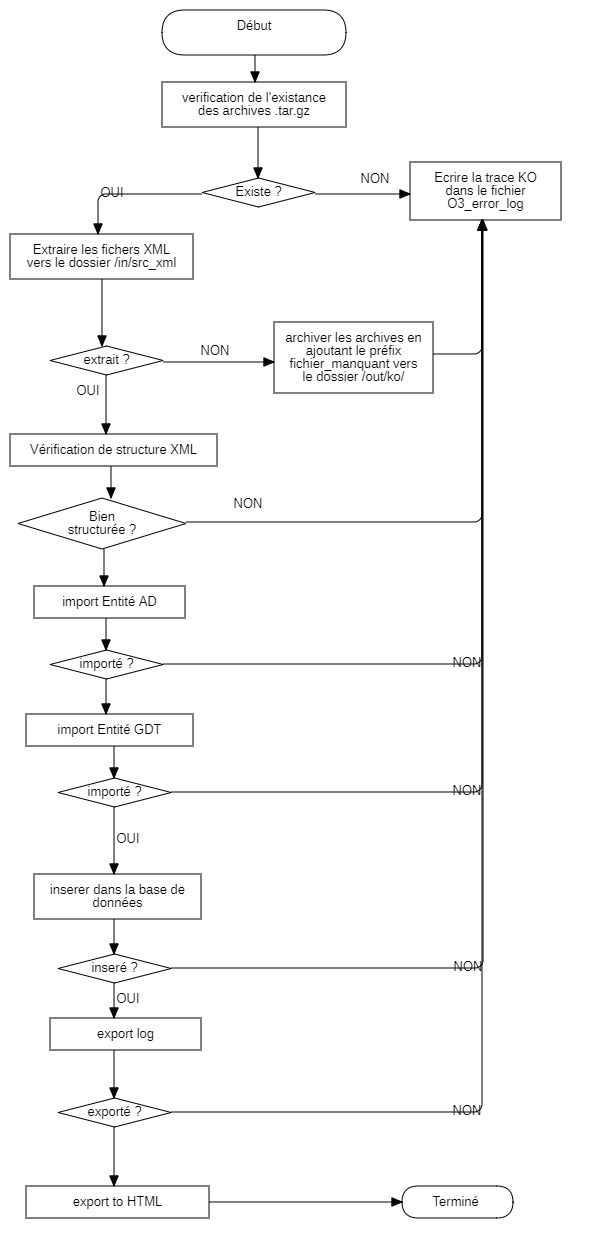
\includegraphics[width=0.5\linewidth]{img/conception/FlowchartDiagram-update-boutique}
	\caption[L'algorigramme de «mise à jour des données boutiques»]{L'algorigramme de «mise à jour des données boutiques»}
	\label{fig:flowchartdiagram-update-boutique}
\end{figure}
\newpage
%===================== ANNEXE 2 =====================%
\section*{Annexe 2.~Entreprise}
\addcontentsline{toc}{section}{Annexe 2.~Entreprise}

\addcontentsline{lof}{figure}{Annexe 2.1~~~Logo d'entreprise}

La figure annexe 2.1 présente le logo entreprise.
\begin{figure}[htpb]
    \centering
    \frame{\includegraphics[width=0.45\columnwidth]{Logo_Entreprise}}
    {\\\textbf{Figure annexe 2.1:} Logo d'entreprise}
\end{figure}

